% 1982 年全国卷（文科）第 9 题：△AOB 中作 AB₁⊥OB、B₁A₁∥BA，再作 A₁B₂⊥OB、B₂A₂∥BA，如此无限作下去；图中 OB 画成竖直线，故垂线 AB₁、A₁B₂、A₂B₃ 为水平线，阴影自下而上依次为 △ABB₁、△A₁B₁B₂、△A₂B₂B₃（按源卷布局）
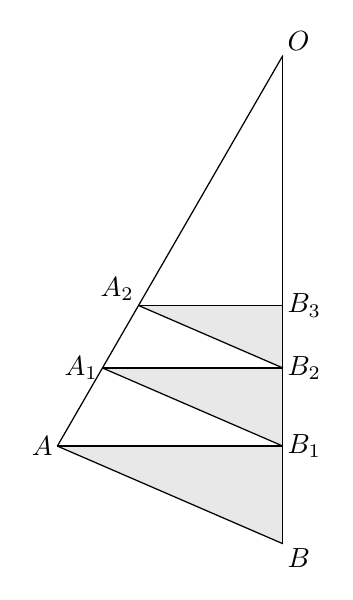
\begin{tikzpicture}[scale=0.62, line width=0.45pt,
  every node/.style={inner sep=1.5pt}]
  % OB 竖直（长 10），OA=b=9.238、∠AOB=θ=30°，公比 k=b·cosθ/a=0.8
  \coordinate (O)  at (0,10);
  \coordinate (B)  at (0,0);
  \coordinate (A)  at (-4.619,2.0);
  \coordinate (B1) at (0,2.0);
  \coordinate (A1) at (-3.695,3.6);
  \coordinate (B2) at (0,3.6);
  \coordinate (A2) at (-2.956,4.88);
  \coordinate (B3) at (0,4.88);
  % 阴影三角形（自下而上依次为 S₁、S₂、S₃）
  \fill[gray!18] (A) -- (B) -- (B1) -- cycle;
  \fill[gray!18] (A1) -- (B1) -- (B2) -- cycle;
  \fill[gray!18] (A2) -- (B2) -- (B3) -- cycle;
  % 各边
  \draw (O) -- (B);
  \draw (O) -- (A);
  \draw (A) -- (B);
  \draw (A) -- (B1);
  \draw (A1) -- (B1);
  \draw (A1) -- (B2);
  \draw (A2) -- (B2);
  \draw (A2) -- (B3);
  % 顶点标注
  \node[anchor=south west] at (O)  {$O$};
  \node[anchor=north west] at (B)  {$B$};
  \node[anchor=east]       at (A)  {$A$};
  \node[anchor=east]       at (A1) {$A_1$};
  \node[anchor=south east] at (A2) {$A_2$};
  \node[anchor=west]       at (B1) {$B_1$};
  \node[anchor=west]       at (B2) {$B_2$};
  \node[anchor=west]       at (B3) {$B_3$};
\end{tikzpicture}
